\section{Phương pháp Thực hiện}
\label{sec:phuongphap}

\subsection{Chương 1 -- Mô hình hóa Kripke \& Kiểm chứng BMC}
\label{sec:ch1}

\textbf{Module:} \texttt{ch1\_models/kripke\_bmc.py}.

Kripke structure $M = (S, S_0, R, L)$ được dựng với \textbf{6 trạng thái ở bản FIXED} ($S_0$ INIT $\to$ $S_1$ GV\_ASSIGNED $\to$ \{$S_{2A}$ CALC\_THUONG $\mid$ $S_{2B}$ CALC\_DONG\} $\to$ $S_3$ EXPORTED, và $S_4$ ERROR) và \textbf{7 trạng thái ở bản BUGGY} (thêm $S_5$ INVALID\_CALC -- đường tắt nhảy trực tiếp từ $S_0$ sang tính tiền, bỏ qua bước phân công giảng viên). \Cref{fig:kripke} minh họa sơ đồ chuyển trạng thái cùng kết quả BMC $P_1$--$P_4$ trên phiên bản gốc trước khi bổ sung $P_5$ và tách $S_{2A}$/$S_{2B}$ (xem giải thích dưới hình và bảng kết quả cập nhật đầy đủ tại \Cref{sec:ketqua}).

Hai trạng thái $S_{2A}$ CALC\_THUONG và $S_{2B}$ CALC\_DONG (thay cho 1 $S_2$ SALARY\_CALC duy nhất trước đây) mô hình hóa đúng nhánh rẽ \emph{thật} trong \texttt{tinh\_tien\_day.c}: \texttt{heSoQuyMo = (soLuongSinhVien > 50) ? 0.2 : 0.0} -- tức là kết hợp \textbf{2 tham số đầu vào} \texttt{soTiet} và \texttt{soLuongSinhVien} thành 1 tham số tổng hợp \texttt{soTietQuyDoi} \emph{tăng dần theo cả hai tham số} (xem chứng minh đơn điệu tại \Cref{sec:params}), và vì \emph{rất nhiều} giá trị \texttt{soLuongSinhVien} khác nhau ($0..50$ hoặc $51..300$) cùng rơi vào 1 trong 2 trạng thái này, mỗi trạng thái được gắn với đúng 1 \textbf{statement} (predicate) tường minh:
\begin{align*}
  S_{2A}\text{ CALC\_THUONG} &\equiv (0 \le \text{soLuongSinhVien} \le 50) \\
  S_{2B}\text{ CALC\_DONG} &\equiv (\text{soLuongSinhVien} > 50)
\end{align*}
Cả 2 nhánh đều mang nhãn \texttt{assigned}+\texttt{calculated} như nhau nên không làm thay đổi kết quả $P_1$--$P_5$ (đã xác nhận lại bằng cách chạy lại BMC sau khi sửa, xem \Cref{sec:ketqua}) -- việc tách trạng thái phục vụ tính \emph{truy vết tường minh} giữa mô hình điều khiển định tính (Kripke) và ràng buộc số học định lượng đã sửa ở Check 1/2 (Z3, \Cref{sec:ch3}), không phải để tạo thêm phát hiện lỗi mới.

\begin{figure}[H]
  \centering
  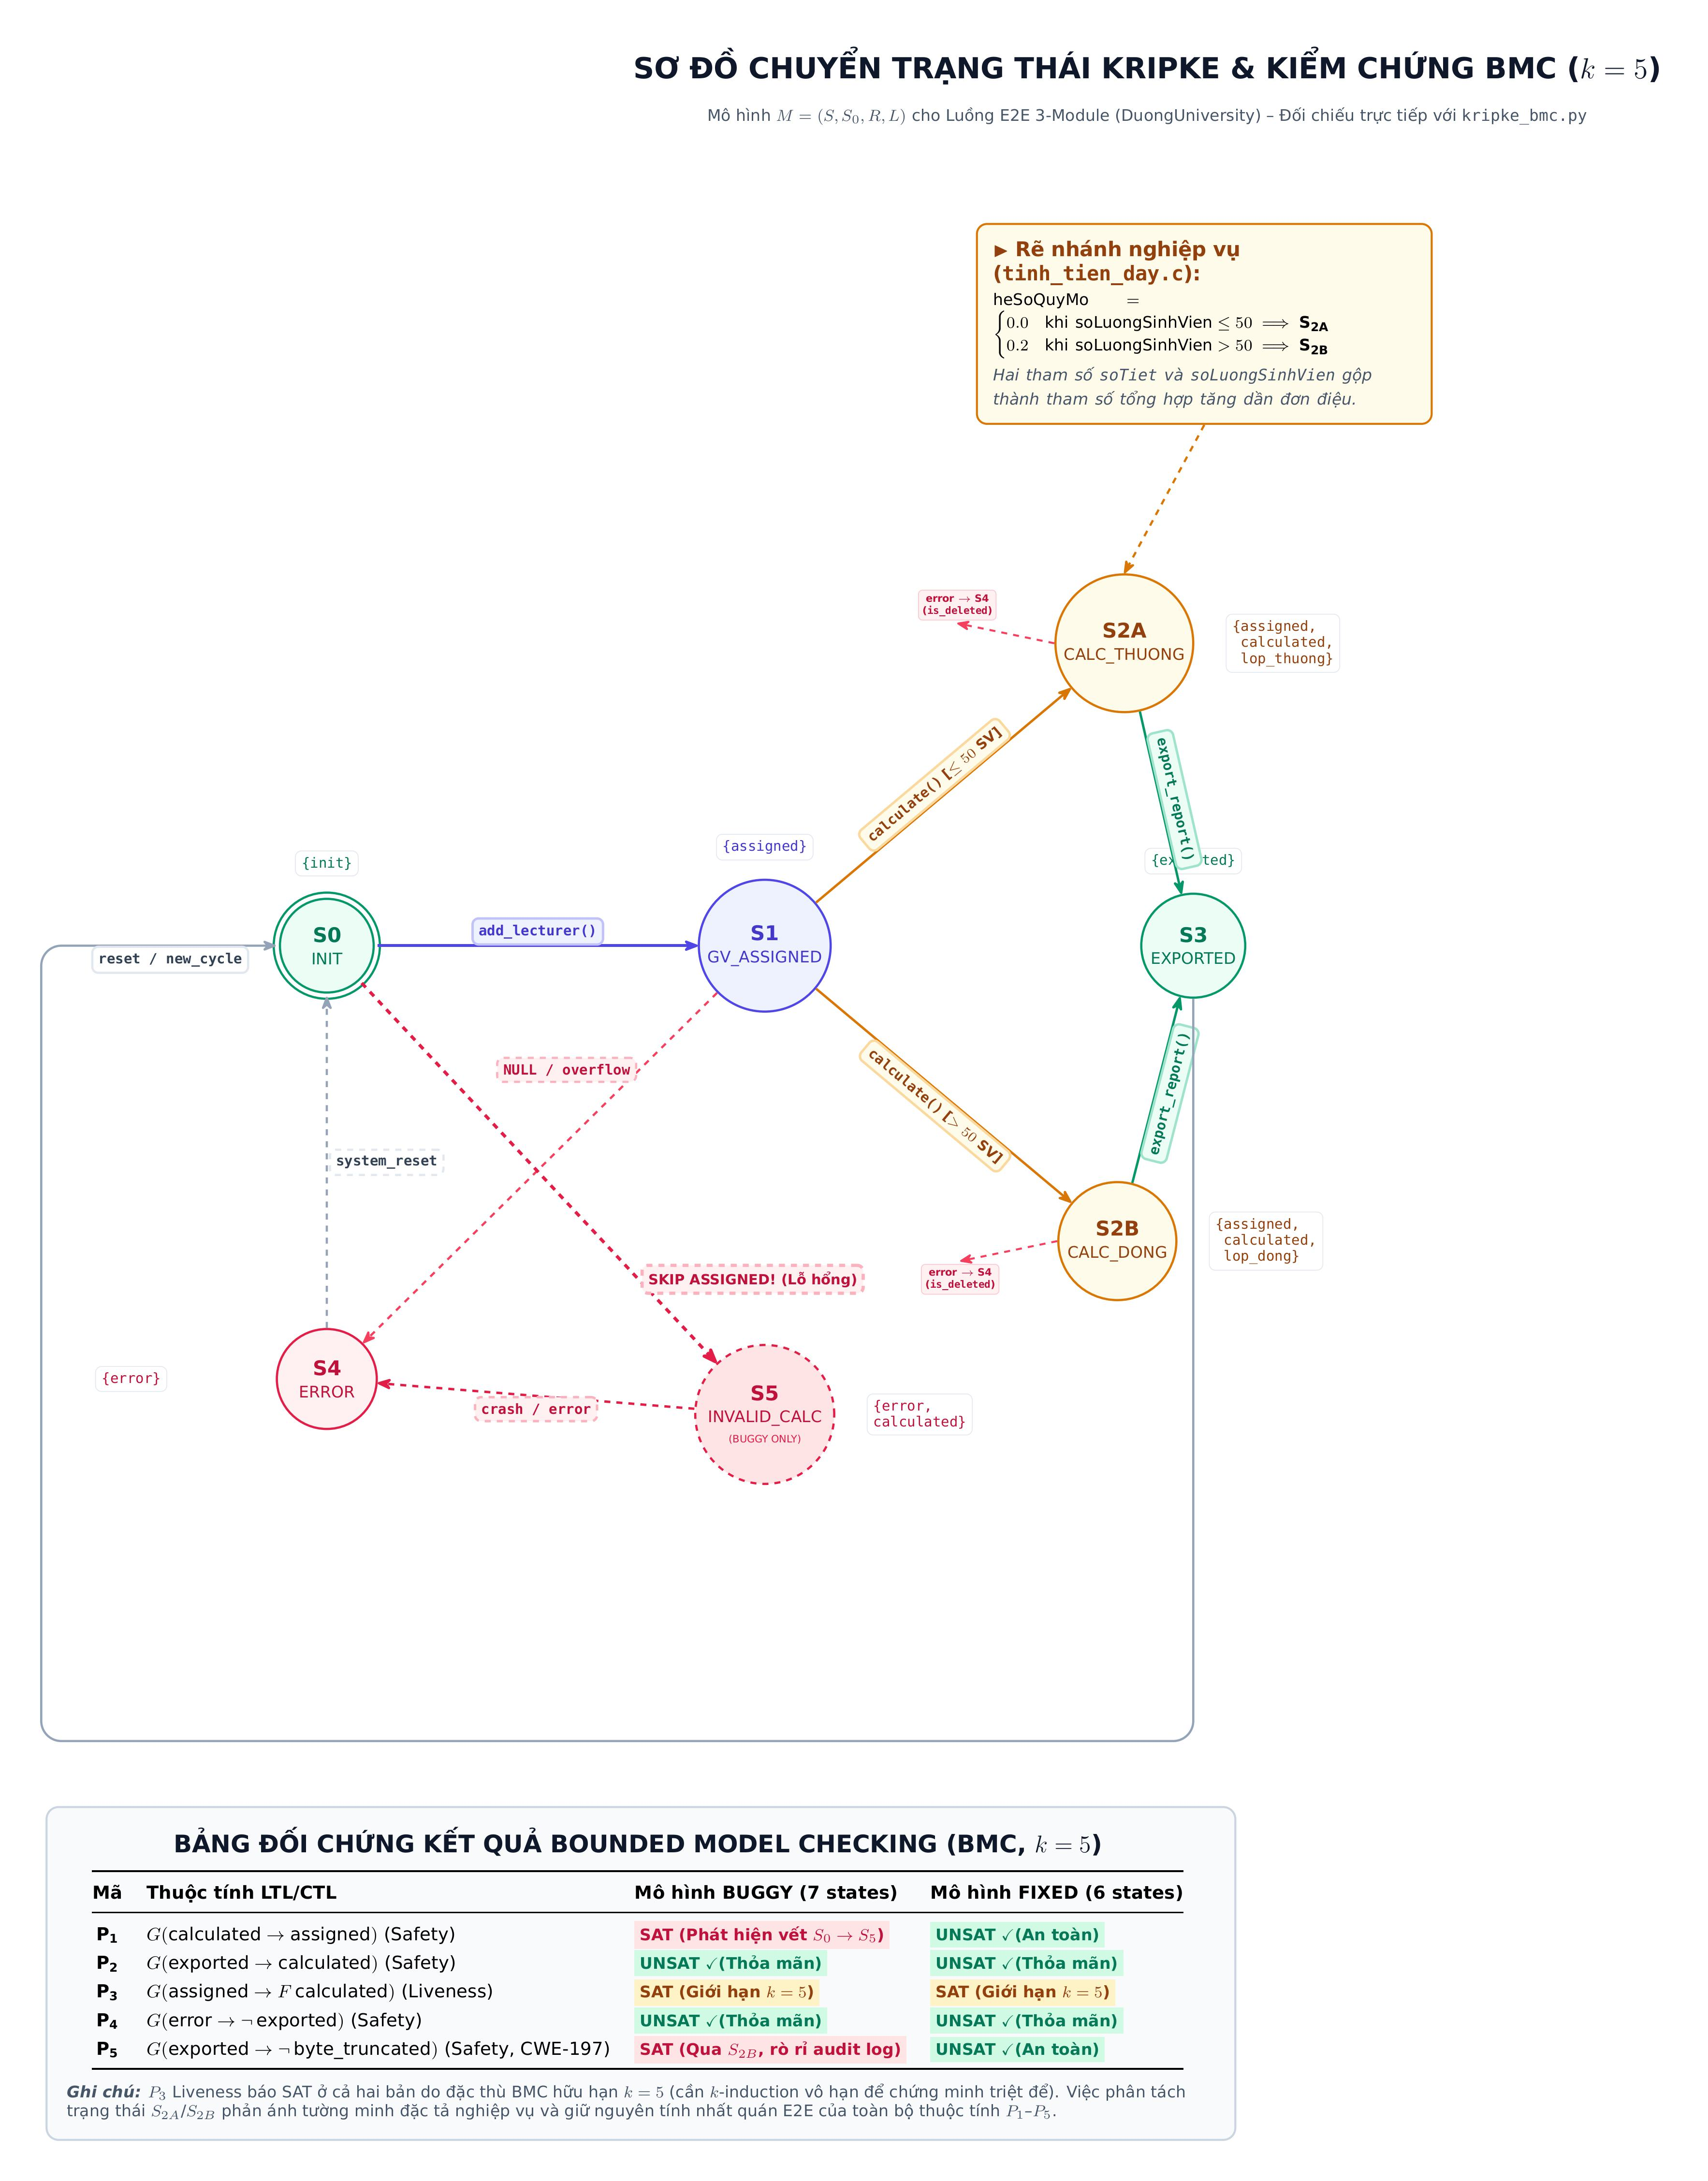
\includegraphics[width=\linewidth]{diagram1_state_transition_fixed.png}
  \caption{Sơ đồ chuyển trạng thái Kripke và kết quả BMC $k=5$ (thuộc tính $P_1$--$P_4$; hình vẽ ở phiên bản gốc trước khi bổ sung $P_5$ và tách $S_2$ thành $S_{2A}$/$S_{2B}$ -- xem văn bản và \Cref{sec:ketqua} để có mô hình và bảng kết quả đầy đủ, cập nhật)}
  \label{fig:kripke}
\end{figure}

\textbf{5 thuộc tính LTL/CTL} được kiểm chứng bằng BMC với $k=5$:
\begin{itemize}
  \item $P_1$ (Safety): $G(\text{calculated} \to \text{assigned})$ -- chưa phân công thì không được tính tiền.
  \item $P_2$ (Safety): $G(\text{exported} \to \text{calculated})$ -- chưa tính tiền thì không được xuất báo cáo.
  \item $P_3$ (Liveness): $G(\text{assigned} \to F\,\text{calculated})$ -- đã phân công thì cuối cùng phải tính tiền.
  \item $P_4$ (Safety): $G(\text{error} \to \lnot\,\text{exported})$ -- hệ thống lỗi thì không được xuất báo cáo.
  \item $P_5$ (Safety, bổ sung cho CWE-197): $G(\text{exported} \to \lnot\,\text{byte\_truncated})$ -- báo cáo xuất ra không được mang dữ liệu ép kiểu sai lệch.
\end{itemize}

Hàm \texttt{cross\_validate\_with\_pattern\_scanner()} gọi lại chính \texttt{pattern\_scanner.py} của Chương 2 để tự động xác nhận trạng thái lỗi $S_4$/$S_3$\_EXPORTED\_TRUNCATED trong mô hình Kripke trừu tượng khớp với đúng vị trí lỗ hổng thật trên mã nguồn C -- liên kết Chương 1 $\leftrightarrow$ Chương 2, tránh việc mô hình hình thức tồn tại độc lập, tách rời code thật.

\subsection{Chương 2 -- Kiểm toán an toàn bộ nhớ}
\label{sec:ch2}

\textbf{Module:} \texttt{ch2\_memsafe/pattern\_scanner.py}.

Công cụ quét trực tiếp mã nguồn C dạng văn bản (regex/so khớp chuỗi, không phải phân tích AST/data-flow đầy đủ) trên 3 file \texttt{giang\_vien.c}, \texttt{lop\_hoc\_phan.c}, \texttt{tinh\_tien\_day.c} và driver \texttt{main\_fixed.c}, với 5 quy tắc phát hiện: \texttt{strcpy} (CWE-120), \texttt{dangling\_free} (CWE-416), \texttt{unchecked\_nested\_deref} (CWE-476), \texttt{int\_overflow\_cast} (CWE-190), \texttt{unchecked\_numeric\_truncation} (CWE-197). Phạm vi tìm ``đã được bảo vệ'' (guard-check) được scope đúng theo \emph{hàm bao quanh} thay vì cửa sổ N dòng cố định, tránh bỏ sót guard nằm xa vị trí truy cập trong hàm dài.

\textbf{Bổ sung bằng chứng động (\texttt{memory\_trace\_demo.py}):} phân tích tĩnh không thể trả lời câu hỏi ``bộ nhớ thực sự được dùng ra sao khi chương trình chạy''. Script này biên dịch cùng một luồng E2E 7 bước bằng 2 trình biên dịch: \textbf{Plain GCC} (chỉ in địa chỉ con trỏ thật, không phát hiện lỗi) và \textbf{Clang64 + AddressSanitizer thật}~\cite{clangasan} (công cụ độc lập tự phát hiện \texttt{heap-use-after-free}), cho phép đối chiếu hành vi ``im lặng'' (nguy hiểm) và hành vi ``bị công cụ chặn'' trên cùng một lỗi.

\subsection{Chương 3 -- Kiểm chứng hình thức SMT/Z3}
\label{sec:ch3}

\textbf{Module:} \texttt{ch3\_staticsat/smt\_verify.py}.

Khác với test thông thường (thử một vài input), Z3 SMT solver~\cite{demoura2008z3} chứng minh một mệnh đề đúng/sai trên \emph{toàn miền giá trị hợp lệ} cùng lúc, với 7 phép kiểm chứng:

\begin{itemize}
  \item \textbf{Check 1}: $\exists$ input hợp lệ ($\text{numClasses}\in[1,20]$, $\text{soTiet}\in[15,120]$, $\text{soLuongSinhVien}\in[0,300]$,\dots) : $\text{tienDay} > \text{INT32\_MAX}$? $\Rightarrow$ \textbf{SAT} -- CWE-190 có thật.
  \item \textbf{Check 2}: cùng câu hỏi với ngưỡng \texttt{INT64\_MAX} trên kiểu \texttt{long long} $\Rightarrow$ \textbf{UNSAT} -- an toàn tuyệt đối.
  \item \textbf{Check 3}: $\text{gv\_ptr} = \text{NULL} \lor \text{is\_deleted} \to \text{tienDay} = 0$? -- mô hình hóa bằng \emph{đúng công thức thật} trong \texttt{calculate\_e2e\_salary\_SAFE()} $\Rightarrow$ \textbf{UNSAT} -- guard hoạt động đúng.
  \item \textbf{Check 4}: $\exists\, \text{soLuongSinhVien}\in[0,300]$ : ép kiểu \texttt{(char)} (mô phỏng bằng số học modulo 256) cho giá trị khác giá trị gốc? $\Rightarrow$ \textbf{SAT} -- phản ví dụ $128 \to -128$.
  \item \textbf{Check 5}: cùng câu hỏi nhưng với guard $0 \le n \le 127$ đứng trước $\Rightarrow$ \textbf{UNSAT} -- chứng minh bản vá loại trừ hoàn toàn CWE-197.
  \item \textbf{Check 6}: $\exists\, a \ne b \in [0,300]$ : ép kiểu cho ra cùng 1 byte? $\Rightarrow$ \textbf{SAT} -- phản ví dụ $a=0, b=256$ cùng cho byte $=0$ (lớp nguy hiểm nhất: 2 lớp học hoàn toàn khác nhau bị nhầm thành một).
  \item \textbf{Check 7} (mới, CWE-1288): $\exists$ 2 danh mục \texttt{bangCap} khác nhau (\texttt{CU\_NHAN} thật, và 1 chuỗi không hợp lệ) : cho cùng 1 \texttt{heSoBangCap}? $\Rightarrow$ \textbf{SAT} -- cả hai cùng rơi vào nhánh fallback $1.0$ của if-chain thật trong \texttt{add\_lecturer\_*()} (xem statement đầy đủ tại \Cref{sec:quytrinh}).
\end{itemize}

Các ràng buộc nghiệp vụ dùng đúng con số đã đặc tả tại \Cref{tab:range} ($\text{soTiet}\in[1,500]$, $\text{dinhMucTienChuan}\in[50\,000,200\,000]$ VNĐ).

\textbf{Một lỗi mô hình đã được tìm và sửa ở Check 1/2:} bản gốc mô hình hóa hệ số quy mô lớp bằng 1 biến \texttt{Real} \emph{tự do} \texttt{heSoQuyMoLop} $\in[0.1,0.5]$/$[0.1,2.0]$, đặt tên theo field \texttt{Config.heSoQuyMoLop} (\texttt{tinh\_tien\_day.h:8}) -- nhưng field này \textbf{không bao giờ được code C thật đọc} (\texttt{tinh\_tien\_day.c} không có \texttt{cfg->heSoQuyMoLop} ở đâu cả, xem đối chiếu tại \Cref{sec:params}), nên phần chứng minh trước đây không phản ánh đúng công thức chạy thực tế. Đã sửa bằng cách thêm \texttt{soLuongSinhVien} là biến Z3 thật và định nghĩa \texttt{heSoQuyMo = If(soLuongSinhVien > 50, 0.2, 0.0)} -- đúng \emph{statement} thật trong code, không phải biến tự do. Sau khi sửa, Check 1 vẫn \textbf{SAT} và Check 2 vẫn \textbf{UNSAT} (kết luận định tính không đổi), nhưng phản ví dụ của Check 1 nay là bộ giá trị mà mô hình sửa vẫn có thể thật sự sinh ra từ code, xem số liệu cập nhật tại \Cref{sec:ketqua}.

\subsection{Chương 4 -- Dynamic Fuzzing}
\label{sec:ch4}

\textbf{Module:} \texttt{ch4\_dynafuzz/fuzzer\_blackbox.py} và \texttt{fuzzer\_whitebox.py}.

\textbf{Black-box}: sinh 200 input ngẫu nhiên (tên/bằng cấp/mã lớp qua \texttt{stdin}), đo crash rate thật trên \texttt{salary\_calc.exe} (VULN) đối chứng \texttt{salary\_calc\_fixed.exe} (SAFE). Riêng CWE-197 được fuzz qua subcommand \texttt{e2e\_byte\_truncate <n>} với 2 chiến lược: (a) 200 giá trị ngẫu nhiên trong $[-50,400]$, và (b) \textbf{Boundary Value Analysis} -- 17 giá trị biên \emph{thiết kế sẵn} (quanh mép \texttt{char} $\{-129,\dots,129\}$, quanh mép chu kỳ 256 $\{-256,\dots,257\}$, và giá trị lớp đại cương $\{300,384\}$) chạy tất định thay vì phó mặc ngẫu nhiên -- đảm bảo luôn phát hiện được lớp lỗi nguy hiểm nhất (trùng lặp byte).

\textbf{White-box (Z3-guided)}: giải trực tiếp 7 ràng buộc Z3 tương ứng 6 lỗ hổng CWE đã biết trước (không phải symbolic execution duyệt CFG tự động) -- hằng số \texttt{MAX\_NAME}/\texttt{MAX\_MALOP} được đọc trực tiếp từ header \texttt{.h} qua \texttt{read\_header\_define()} thay vì hard-code, nên ràng buộc Z3 tự động bám theo đúng source hiện tại nếu hằng số đổi.
